\begin{frame}[fragile]
  \frametitle{Simple screen scraping}

    \begin{block}{One-liner to scrape images from a webpage}
        \begin{lstlisting}[language=bash]
 wget -O- http://bit.ly/gpCSQi | 
   tr ''\''"=' '\n' | 
   egrep '^http.*(png|jpg|gif)' | 
   xargs wget 
        \end{lstlisting}
    \end{block} 

    \pause
    \begin{itemize}
      \item get page source
      \item translate quotes and = to newlines
      \item match urls with image extensions
      \item download qualifying images
    \end{itemize}

\end{frame}


\begin{frame}
  \frametitle{``cat flickr \big| xargs wget''?}

  \begin{center}
    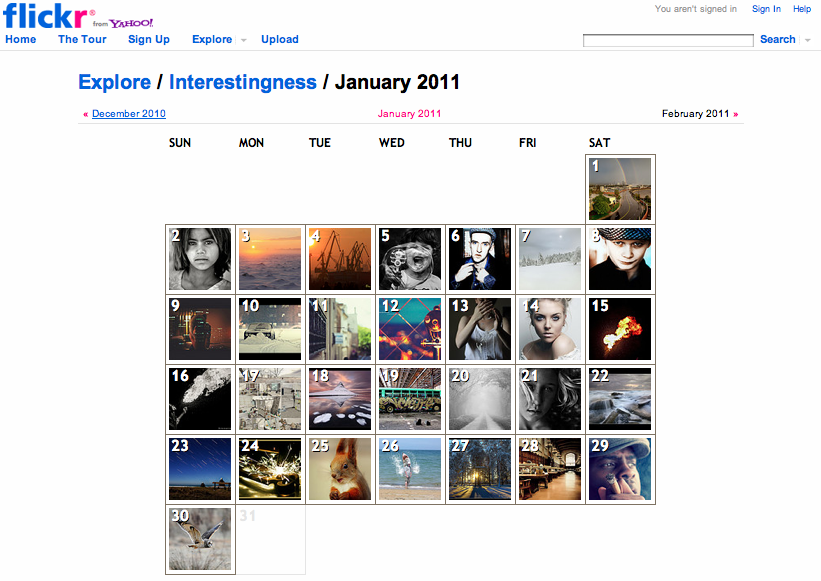
\includegraphics[width=\textwidth]{flickr_201101.png}
  \end{center}

\end{frame}


\begin{frame}
  \frametitle{Flickr API}

  \begin{center}
    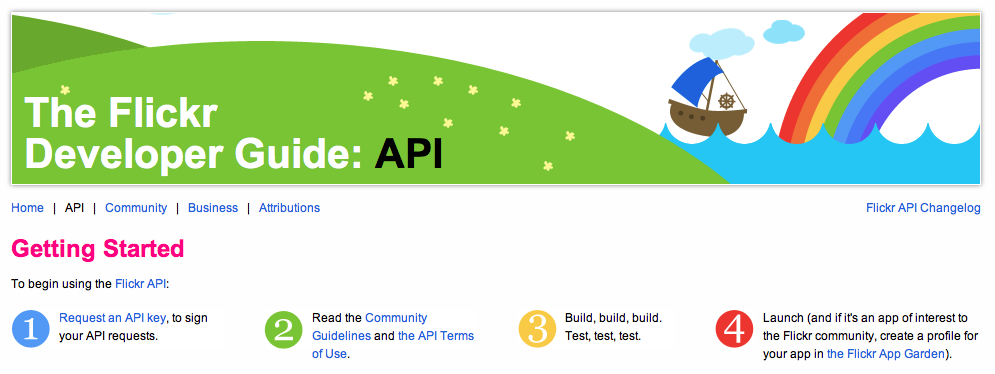
\includegraphics[width=\textwidth]{flickr_api.png}
  \end{center}

\end{frame}


\begin{frame}
  \frametitle{SELECT * FROM Internet\footnote{\url{http://oreillynet.com/pub/e/1369}}}

  \begin{center}

    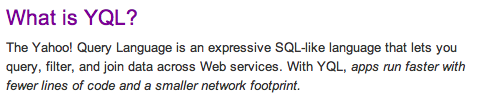
\includegraphics[width=\textwidth]{what_is_yql.png}
    \url{http://developer.yahoo.com/yql}

  \end{center}

\end{frame}


\begin{frame}
  \frametitle{YQL Console}

  \begin{center}
    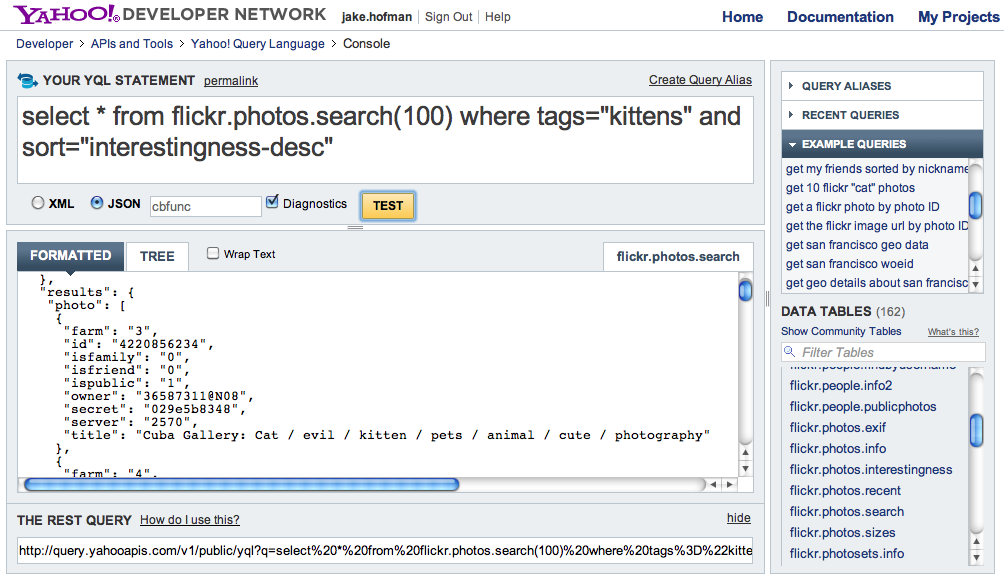
\includegraphics[width=\textwidth]{yql_console.png}
    \url{http://developer.yahoo.com/yql/console}
  \end{center}

\end{frame}


\begin{frame}[fragile]
  \frametitle{YQL + Python\footnote{See \url{http://python-yql.org/} for a more robust client}}

    \begin{block}{Python function for public YQL queries}
        \begin{lstlisting}[language=python]
YQL_PUBLIC = 'http://query.yahooapis.com/v1/public/yql'

def yql_public(query):
  # escape query
  query_str = urlencode({'q': query, 'format': 'json'})

  # fetch results
  url = '%s?%s' % (YQL_PUBLIC, query_str)
  result = urlopen(url)

  # parse json and return
  return json.load(result)['query']['results']

        \end{lstlisting}
    \end{block}
\end{frame}

\begin{frame}[fragile]
  \frametitle{YQL + Python + Flickr}

    \begin{block}{Fetch info for ``interestingness'' photos}
      \begin{lstlisting}[language=bash]
 ./simpleyql.py ``select * from
   flickr.photos.interestingness(100)''
      \end{lstlisting}
    \end{block}

    \begin{block}{Download thumbnails for photos tagged with ``vivid''}
      \begin{lstlisting}[language=bash]
 ./download_flickr.py vivid 500
      \end{lstlisting}
    \end{block}

\end{frame}
